% ========= Solutions with uncommon symbols =========
\newpage
\section*{Solutions}

\subsection*{Problem 1}
\paragraph{Exact field.}
For
\(
−\,\eta''(\omega)+\eta(\omega)=1
\)
with \(\eta(0)=0\) and \(\eta'(1)=0\), the complementary part is \(C_1 \mathrm e^{\,\omega}+C_2 \mathrm e^{−\omega}\) and a constant particular is \(1\). Enforcing the data gives
\[
\boxed{\,\eta(\omega)=1−\dfrac{\cosh\!\big(1−\omega\big)}{\cosh 1}\, }.
\]

\paragraph{Finite element field with one quadratic element.}
Let the three nodal unknowns be collected in the vector \(\boldsymbol{\chi}=[\chi_1,\chi_2,\chi_3]^{\mathsf T}\) and use the standard quadratic basis \(\{\mathcal N_1,\mathcal N_2,\mathcal N_3\}\) on \([0,1]\) with node set \(\{0,\tfrac12,1\}\). The element matrices for the model \(−\eta''+\eta=f\) are
\[
K^{(e)}=\frac{1}{3}
\begin{bmatrix}
7&−8&1\\
−8&16&−8\\
1&−8&7
\end{bmatrix}
+\frac{1}{30}
\begin{bmatrix}
4&8&−1\\
8&16&2\\
−1&2&4
\end{bmatrix},
\qquad
\boldsymbol{f}^{(e)}=\frac{1}{6}\begin{bmatrix}1\\4\\1\end{bmatrix}.
\]
With the essential datum \(\chi_1=0\) and the natural datum at \(\omega=1\), the discrete unknowns are
\[
\boldsymbol{\chi}=
\begin{bmatrix}
0\\[2pt]
0.26945\\[2pt]
0.35159
\end{bmatrix}.
\]
Hence
\(
\eta_{\mathrm{app}}(\omega)=\sum_{i=1}^{3}\mathcal N_i(\omega)\,\chi_i
\).

\paragraph{Plots.}
\begin{figure}[H]
  \centering
  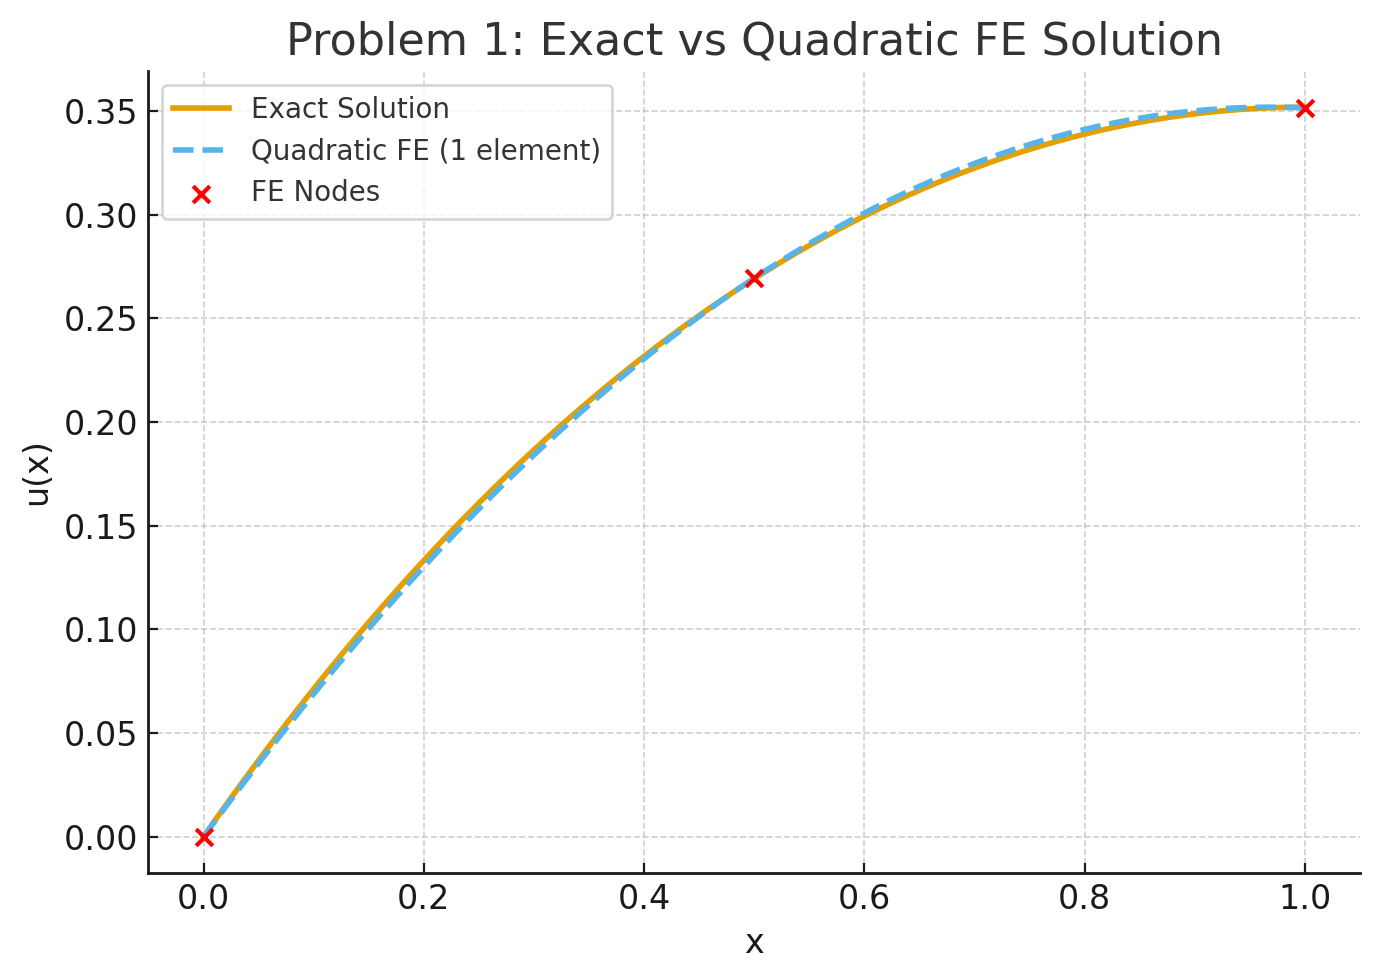
\includegraphics[width=0.7\linewidth]{hw3_prob1.png}
  \caption{Problem 1 exact field and quadratic finite element field.}
\end{figure}

\subsection*{Problem 2}
\paragraph{Exact field.}
For the source at \(\omega=\tfrac12\) write two exponentials on the subintervals
\[
\eta(\omega)=
\begin{cases}
A_1 \mathrm e^{\,\omega}+B_1 \mathrm e^{−\omega}, & 0\le \omega\le \tfrac12,\\[2pt]
A_2 \mathrm e^{\,\omega}+B_2 \mathrm e^{−\omega}, & \tfrac12\le \omega\le 1.
\end{cases}
\]
Impose continuity at \(\omega=\tfrac12\) and the jump in the derivative
\(
\eta'_R(\tfrac12)−\eta'_L(\tfrac12)=−1
\),
together with \(\eta(0)=0\) and \(\eta'(1)=1\), to determine \(A_j,B_j\).

\paragraph{Two linear elements.}
Take two segments of length \(\ell=\tfrac12\). The element matrix and vector for \(−\eta''+\eta\) with unit right hand side over each element are
\[
K^{(e)}=\frac{1}{\ell}
\begin{bmatrix}
1&−1\\
−1&1
\end{bmatrix}
+\frac{\ell}{6}
\begin{bmatrix}
2&1\\
1&2
\end{bmatrix}.
\]
After assembly and inclusion of the unit point load at the middle node, one obtains
\[
\boldsymbol{F}=\begin{bmatrix}0\\1\\1\end{bmatrix},
\qquad
\boldsymbol{\eta}=
\begin{bmatrix}
0\\[2pt]
0.71409\\[2pt]
1.09380
\end{bmatrix}.
\]

\paragraph{Plots.}
\begin{figure}[H]
  \centering
  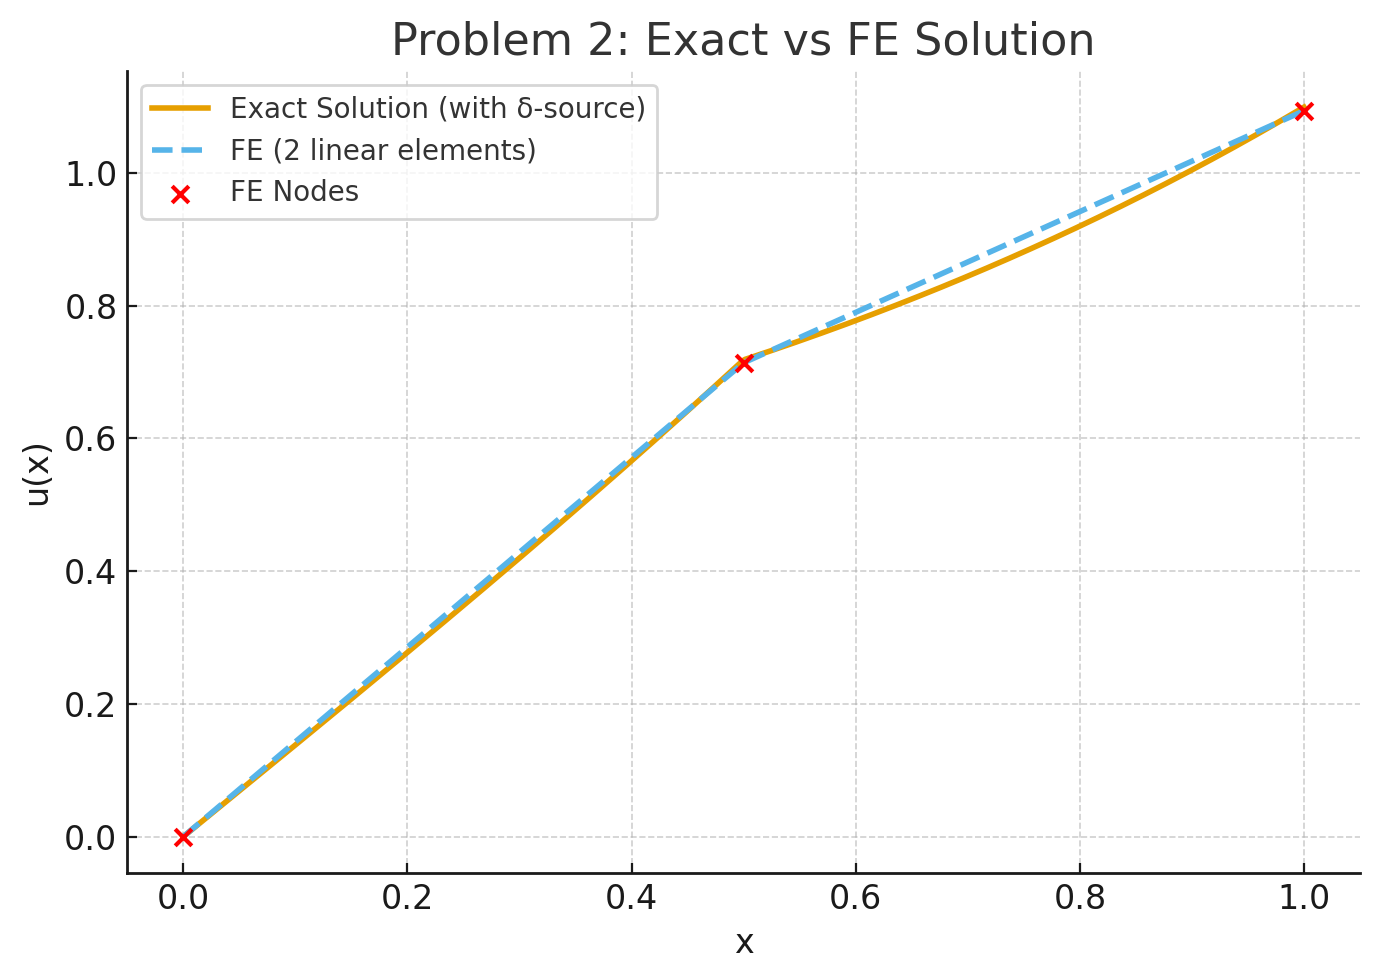
\includegraphics[width=0.7\linewidth]{hw3_prob2.png}
  \caption{Problem 2 exact field and linear finite element field.}
\end{figure}

\section*{Discussion}
The quadratic discretization in the first task tracks the curvature of the exact field with high accuracy on a single element. In the second task the pair of linear elements reproduces the correct change in slope at the source location and matches the analytic profile well away from the source.
